\documentclass[tikz,border=2pt]{standalone}
\usepackage{amsmath,amssymb}
\usepackage{tikz}
\usetikzlibrary{arrows.meta}

\begin{document}
% The length b-a does not depend on whether the endpoints are included: [a,b], (a,b), [a,b)
% and (a,b] all have the same length.
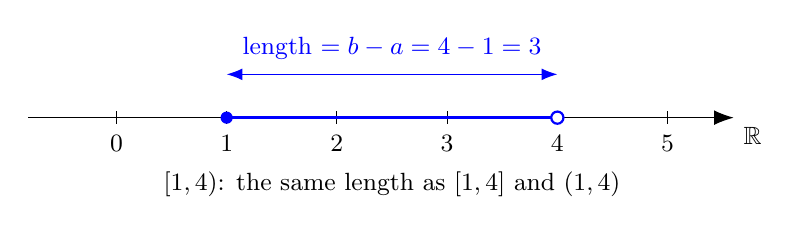
\begin{tikzpicture}[x=1.4cm, every node/.style={font=\small}]
	\draw[-{Latex[length=2.5mm]}] (-0.8,0) -- (5.6,0) node[below right] {$\mathbb{R}$};
	\foreach \x in {0,1,2,3,4,5} {\draw (\x,0.08) -- (\x,-0.08); \node[below=3pt] at (\x,0) {$\x$};}
	\draw[very thick, blue] (1,0) -- (4,0);
	\fill[blue] (1,0) circle (2.2pt);
	\draw[blue, thick, fill=white] (4,0) circle (2.2pt);
	\draw[blue, {Latex[length=2mm]}-{Latex[length=2mm]}] (1,0.55) -- (4,0.55);
	\node[blue, above=2pt] at (2.5,0.55) {length $=b-a=4-1=3$};
	\node[below=16pt] at (2.5,0) {$[1,4)$: the same length as $[1,4]$ and $(1,4)$};
\end{tikzpicture}
\end{document}
